\documentclass[journal,twoside]{IEEEtran}

%% Citations
\usepackage{cite}
%\usepackage[sort&compress]{natbib}
%\bibpunct{[}{]}{,}{n}{,}{,}

%% AMS
\usepackage[cmex10]{amsmath}
\usepackage{amssymb,amsfonts}
\interdisplaylinepenalty=2500

%% Balance columns
%\usepackage{balance}

%% Better arrays
\usepackage{array}

%% Enumeration
\usepackage{enumerate}

%% Figures
\usepackage[pdftex]{graphicx}
\graphicspath{/Figures/}
\DeclareGraphicsExtensions{.png}
\usepackage[section]{placeins}

%% Fix some formatting issues
\usepackage{fixltx2e}
\usepackage{dblfloatfix}

%% Better cross-referencing
\usepackage[capitalize]{cleveref}

%% Newline for paragraphs instead of indenting
%\setlength{\parindent}{0in}
%\setlength{\parskip}{5pt plus 1pt minus 1pt}

\usepackage{threeparttable} % More control over tables

\usepackage{xcolor} % Use this for different colors -- useful for indicating what's changed since last review round
\newcommand{\changed}[1]{\textcolor{red}{#1}}

%% correct bad hyphenation here
\hyphenation{op-tical net-works semi-conduc-tor}

% The paper headers
\markboth{IEEE Transactions on Components, Packaging, and Manufacturing Technology, Vol. ??, No. ??, Month ??, 20??}{Wahby \MakeLowercase{\textit{et al.}}: A Virtual Integration Platform for 2D and 3D IC Design Space Exploration}


\begin{document}
%% fix dashed lines for repeated author names in IEEE style bibliographies
%% NOTE: This requires some fiddling with the bibliography as well
\bstctlcite{IEEEexample:BSTcontrol} 

%% paper title
%% can use linebreaks \\ within to get better formatting as desired
\title{\changed{Investigation of Power, Signal, and Thermal Performance of 2D and 3DICs Using a Novel Virtual Integration Platform}}
\author{William~Wahby,~\IEEEmembership{Student~Member,~IEEE}, Li~Zheng, Yang~Zhang,~\IEEEmembership{Student~Member,~IEEE}, and Muhannad~Bakir,~\IEEEmembership{Senior~Member,~IEEE}%
	\thanks{Original manuscript received July 11, 2015. \changed{Revised manuscript received October ??, 2015.} This work was supported in part by the SRC GRC project 2254.001, and by the SRC Educational Alliance Intel Foundation Fellowship}%
\thanks{William Wahby, Li Zheng, Yang Zhang, and Muhannad Bakir are with the School of Electrical and Computer Engineering, Georgia Institute of Technology, Atlanta, GA, 30332 USA. (emails: wwahby3@gatech.edu; lizheng@gatech.edu; steven.zhang@gatech.edu; muhannad.bakir@mirc.gatech.edu)}}




\maketitle

%\IEEEpeerreviewmaketitle


%% =================================
%% ========== ABSTRACT =============
%% =================================
\begin{abstract}
In order to compare the costs and benefits of 2D and 3DIC technologies, an integrated virtual platform for 3DIC system evaluation and
design space exploration is developed. The virtual platform is implemented in MATLAB, and is composed of several
simulation modules, including a compact 3DIC wire length distribution,
a wire pitch and repeater insertion module, a 2D and 3DIC power supply noise
estimation module, and a finite difference thermal simulator.
The virtual platform is validated against published data for several commercial 2D processors at the 65nm, 45nm, and 32nm nodes.
In order to quantify the benefits both 2D and 3D integration approaches, a 32nm CPU core is modeled and the impact of several
technology parameters, including interlayer dielectric (ILD) material, on-chip wire material, die thickness, 
and cooling solution are explored. 3D integration is shown to provide a significant power reduction for the 32nm test case,
but more aggressive cooling solutions must be employed to maintain the same clock frequency, due to the increased
areal power density of the 3D CPU.
\end{abstract}

\begin{IEEEkeywords}
Three-dimensional integrated circuits, integrated circuit modeling, integrated circuit interconnections, power dissipation.
\end{IEEEkeywords}

%% =================================
%% ======== INTRODUCTION ===========
%% =================================
\section{Introduction}
\IEEEPARstart{E}{conomic} and physical challenges to conventional 2D scaling are driving interest in 3D integration,
but uncertainty regarding the fabrication costs and system-level tradeoffs of 3D integration
complicate 3DIC design. Projections of 3DIC cost and performance are further complicated by the strongly-coupled
nature of communication, power delivery, and thermal management in 3DICs. Additionally, the 3DIC
design space is complex, as 3DIC design encompasses a broad spectrum of possible design choices and integration
methodologies, ranging from 2.5D interposer-based integration all the way to finely-grained monolithic 
3DICs, as shown in \cref{f-3d-spectrum}, each with unique costs and strengths.
% Conventional 2D
% 2.5D - die on interposer
% 3D die stacking with TSVs
% Monolithic 3D
% Blocks stacked on blocks
% Gates stacked on gates
% NFETs and PFETs on separate levels

Additionally, different technologies must be evaluated for use in both 2D and 3DICs.
Low-k dielectrics can be used to reduce the parasitic capacitances in the wiring stack,
simultaneously improving RC delay and reducing the power consumption of the wiring network.
Alternate wiring materials are also being considered to improve the RC delay of on-chip interconnects,
as well as to reduce the risk of electromigration failures. Fluidic cooling can be used to mitigate the thermal challenges
in high performance 2D and 3D ICs. In order to understand the 3D design space, and to decide when a 3D system
might have advantages over a 2D system, all of these factors must be modeled simultaneously.

In order to better understand the tradeoffs inherent in 3DIC design, we present an integrated virtual platform for 3DIC evaluation
to enable rapid exploration of the 3DIC design space. The virtual platform consists of several simulation
modules specially tailored for 3DICs, described in \cref{s-virtual-platform}, which have been interconnected to simultaneously explore the 
signal, power, and thermal behavior of a 3D or 2D system. In order to understand the impact of 3D design on
signaling, a novel compact stochastic wire length model has been developed, which accounts for the TSV-induced
displacement of logic gates in a 3DIC \cite{wahby_wld_2013}. Simple models for wire pitch determination
and repeater insertion are used to develop a complete picture of the on-chip signaling network \cite{venkatesan_performance_1999,bakoglu_optimal_1985}.
The 3DIC power delivery network is also modeled to determine the maximum simultaneous switching noise in the system,
and to understand how many TSVs must be used for power delivery. A multiscale finite difference thermal module
is also included, which rapidly and accurately determines the thermal profile of each layer in a 3D stack.
All of the models can be applied equally well to 2D ICs, allowing for direct comparison of the costs and benefits of 3D integration
and other more conventional technological improvements.

\begin{figure}[!tb]
	\centering
	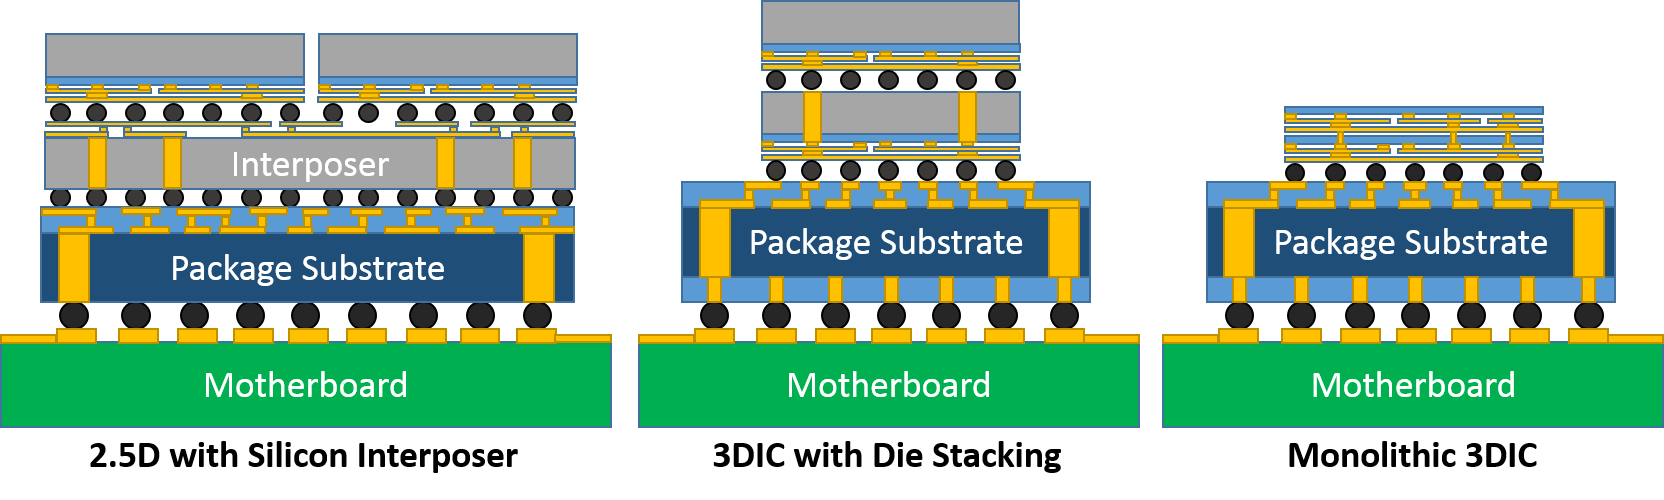
\includegraphics[width=3.5in]{Figures/spectrum_of_3d_4.png}
	\caption{There are many potential configurations for 3DICs, each with their own costs and advantages.
			Designers must manage the complexity of the 3DIC design space in order to achieve higher performance
			and lower cost systems.}
	\label{f-3d-spectrum}
\end{figure}

To ensure the reliability of the virtual platform, its predictions are validated against published data for commercial processors
in \cref{s-validation}.
The virtual platform is used to investigate the impacts of advanced
technologies and integration methodologies on a 32nm Sandy Bridge i7 processing core in \cref{s-2d-investigations,s-3d-investigations}.
Specifically, the impacts of interlayer dielectric material, wire material, and 2D vs 3D integration on the power consumption,
power supply noise, and number of metal layers required for routing are considered.

\section{Virtual Design Platform} \label{s-virtual-platform}
 The virtual platform consists of the following:
 \begin{enumerate}
	\item 3D wire length distribution which properly accounts for TSV area
	\item Metal layer pitch determination algorithms capable of handling alternate wiring materials
	\item An optimal repeater insertion scheme
	\item Power supply noise models which account for power delivery in 3DICs
	\item  A finite difference thermal module for analyzing the thermal impacts of 3D integration
\end{enumerate}

The overall execution flow is shown in \cref{f-vp-flowchart}.
The 3DIC simulation platform can be used to compare the properties of 2D and 3D chips.
Currently, the interconnections between logic blocks are not modeled when simulating heterogeneous (SoC-like) 3D stacks,
which must be taken into account when simulating such systems. In order to better predict the
performance of 3D SoCs, the method of \cite{zarkesh-ha_pin_1998} can be used to homogenize
a heterogeneous system.

\begin{figure}[!tb]
	\centering
	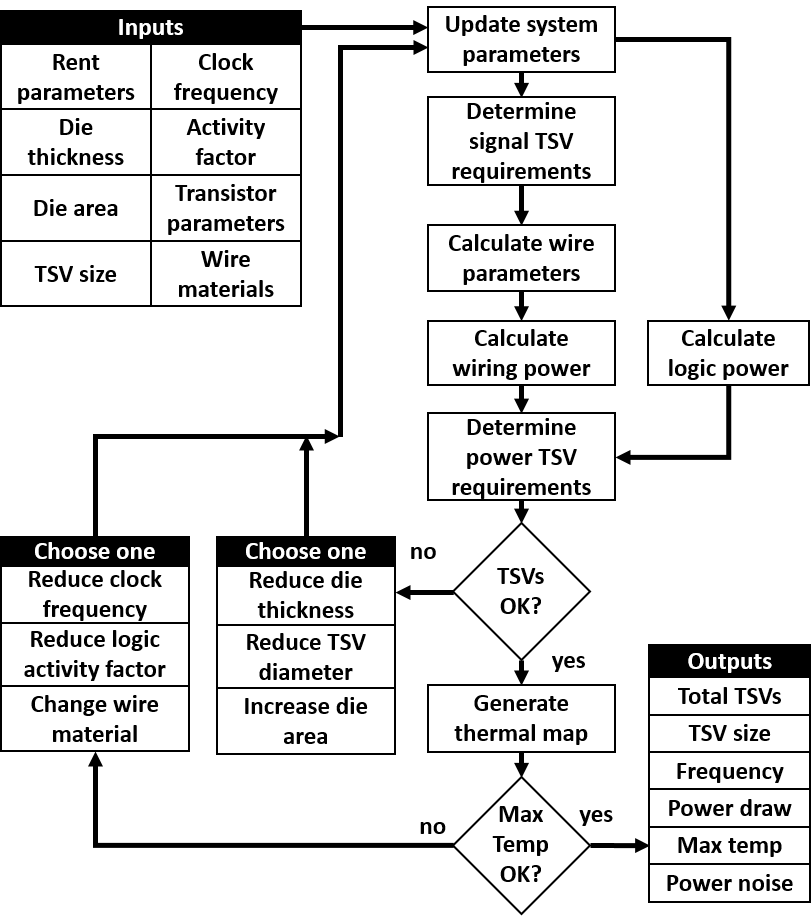
\includegraphics[width=3.5in]{Figures/vp-flowchart-2.png}
	\caption{Block diagram of the virtual platform execution flow.}
	\label{f-vp-flowchart}
\end{figure}


%% =================================
%% ========= Interconnects ============
%% =================================
\subsection{Interconnect modeling}
Stochastic wire length distributions have been shown to be effective tools for the rapid prediction
of interconnect properties in 2D and 3D ICs
\cite{davis_stochastic_1998,davis_stochastic_1998-1,venkatesan_performance_1999,joyner_impact_2001,sekar_intsim_2007}.
 Efforts have been made to extend 2D wire length distributions to 3DICs
\cite{rahman_wire-length_1999-1,joyner_three-dimensional_2000, kim_through-silicon-via_2009-1},
but until recently the impact of TSV diameter on the wire length distribution was difficult to capture.
We recently developed a compact model for the wire length distribution in 3DICs which properly accounts for the
displacement of logic gates by TSVs \cite{wahby_wld_2013}, which has been integrated into the virtual
platform.

Stochastic wire length distributions determine the number of wires of a particular length as
%
\begin{align}
	I_{idf}(l) &= M(l)P_c(l) \label{eq-iidf}
\end{align}
%
where $M(l)$ is the number of gate pairs separated by length $l$, and $P_c(l)$ is the probability that
two gates separated by length $l$ will be connected. The general method of determining $M$ and $P$
in 2D ICs is laid out in \cite{davis_stochastic_1998}. The method was extended to consider 3DICs in
\cite{rahman_wire-length_1999-1,joyner_three-dimensional_2000}, but the impact of TSV-induced gate blockage
was not considered until \cite{kim_through-silicon-via_2009-1} introduced a modified form of $M$ which
accounted for logic displacement, but required brute-force calculation of the correction terms.
This work uses expressions for $M$ and $P$ from \cite{joyner_three-dimensional_2000} with a compact 
correction to $M$ to account for TSV-induced gate displacement \cite{wahby_wld_2013}.

For a symmetric square chip, with a periodic square array of TSVs, the corrected gate pair function is \cite{wahby_wld_2013}:
%
\begin{align}
	M^*_{t}(l) &\cong M_t^o(l,N_s) - 2g \ast g  + N_{tsv}M_t^0(l,N = w_{tsv}^2) \label{eq-mt-corr}
\end{align}
%
where $M_t^o$ is the 2D gate pair separation function described in \cite{joyner_three-dimensional_2000}, $g$ is the 1D inverse
cumulative distribution of {\em potentially} forbidden gate locations \cite{wahby_wld_2013}, $N_{tsv}$ is the
number of TSVs in the logic tier of interest, $N_s$ is the number of logic gates on the tier of interest, $w_{tsv}$ is the
TSV width, and $l$ is the grid distance between two gates.

By substituting \cref{eq-mt-corr} for the 2D gate placement function in \cite{joyner_three-dimensional_2000}, the impact of TSV-induced
logic displacement can be modeled.
The wire pitch and number of metal layers are determined using a bottom-up wire scaling 
technique \cite{venkatesan_performance_1999}, and an optimal repeater insertion scheme 
is used to determine the size and number of repeaters required to meet timing constraints \cite{bakoglu_optimal_1985}.



\subsection{Material considerations}
As interconnect dimensions continue to scale, the properties of wiring materials have begun to diverge from their bulk values.
Surface scattering and grain boundary scattering greatly enhance the resistivity of nanoscale copper wires \cite{sun_surface_2010}.
In order to capture the impact of these effects on wire resistivity, 
we use a combined Mayadas-Shatzke and Fuchs-Sondheimer (MS+FS) model 
\cite{sun_surface_2010,mayadas_electrical-resistivity_1970,fuchs_conductivity_1938,sondheimer_mean_1952}, with
specularity of $0.55$ and backscattering probability of $0.43$ \cite{sun_surface_2010}.
In all cases, the grain size is approximated as the smallest dimension of the wire under consideration.


%% =================================
%% ========= POWER ============
%% =================================

\subsection{Power supply noise modeling}
Power supply noise must be suppressed to ensure reliable system operation, but power delivery in 3DICs is 
complicated by the limited area available for routing power interconnects between tiers.
We use the 3DIC power supply network models developed in \cite{zheng_novel_2014,huang_power_2012}
to determine the maximum power supply noise in the 3D stack and the number of TSVs required for power delivery.

%% =================================
%% ========= THERMAL ============
%% =================================
\subsection{Thermal modeling}
Thermal issues are one of the greatest challenges in 3DIC design.
In order to design a thermally robust 3D system, the relationships between device technology, system performance
area constraints, and packaging materials and technology must be explored.
To that end, we utilize a fast and accurate finite difference thermal model.

The heat transfer equation is
%
	\begin{align}
		\nabla \left( K(x,y,z) \cdot \nabla \left( T(x,y,z) \right) \right) &= P(x,y,z)	\label{eq-heat-transfer}
	\end{align}
%
where $K$ and $T$ denote thermal conductivity and temperature, respectively, and $P$ is the power excitation.
Following the scheme of \cite{xie_electrical-thermal_2011}, we discretize the heat transfer equation as
%
\begin{align}
	&\frac{T_{i,j,k} - T_{i-1,j,k}}{ \frac{x_1}{k_z l_y l_x}} + \frac{T_{i,j,k} - T_{i+1,j,k}}{ \frac{x_2}{k_x l_y l_z}} \nonumber \\ 
	&\quad+ \frac{T_{i,j,k} - T_{i,j-1,k}}{ \frac{y_1}{k_y l_x l_z}} + \frac{T_{i,j,k} - T_{i,j+1,k}}{ \frac{y_2}{k_y l_x l_z}} \nonumber \\
	&\quad+ \frac{T_{i,j,k} - T_{i,j,k-1}}{ \frac{z_1}{k_z l_x l_z}} + \frac{T_{i,j,k} - T_{i,j,k+1}}{ \frac{z_2}{k_z l_x l_z}}  = P_{tot}
\end{align}
%
where $l_x = (x_1+x_2)/2$, $l_y = (y_1+y_2)/2$, $l_z = (z_1+z_2)/2$, and where $x_i$, $y_i$, and $z_i$ ($i \in {1,2}$) are the mesh size
along the corresponding axis. $P$ is the total power consumption in the volume of interest, shown as the shaded rectangular region in
\cref{f-thermal-fdm}. A similar scheme can be derived for grid points along the boundary of the mesh. In the case that
one mesh has multiple materials, we assign the volume-weighted thermal conductivity of the surrounding volume to that grid point.

The accuracy of this finite difference module was assessed in \cite{zhang-thermal-2014}, in which the performance of the finite difference scheme
was compared against finite element ANSYS models of the same structure. The finite difference model was found to match the ANSYS results with a maximum
error of 2.7\%.

\begin{figure}[!htbp]
	\centering
	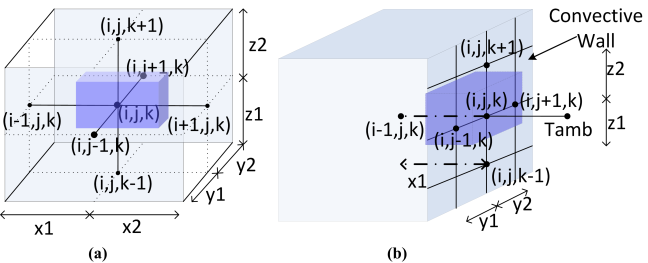
\includegraphics[width=3.5in]{Figures/thermal_fd_setup.png}
	\caption{
		Finite difference scheme. $(a)$ Points inside the stack. $(b)$ Boundary points at the face of the stack \cite{xie_electrical-thermal_2011}.
	}
	\label{f-thermal-fdm}
\end{figure}





%% =================================
%% ========= VALIDATION ============
%% =================================

\section{Validation} \label{s-validation}
The virtual platform was validated by comparing its predictions against published data for Intel processors ranging from the 65nm node
to the 32nm node
\cite{bai_65nm_process_2004,sakran_65nm_merom_arch_2007,mistry_45nm_process_2007,varghese_45nm_penryn_arch_2007,kumar_45nm_nehalem_arch_2009,packan_32nm_process_2009,kurd_32nm_westmere_arch_2010,yuffe_32nm_sandy_arch_2011}.
For each test case, the chip area, number of logic transistors, number of memory transistors, and size and shape
of the cores and memory blocks were gathered from published data. Logic cores were simulated with a Rent exponent of $0.6$,
while memory cores used a value of $0.4$ \cite{christie_interpretation_2000}.
\changed{In cases with integrated GPUs,
the GPU was simulated with a Rent exponent of $0.5$. Each block is simulated separately to determine the number and
pitch of metal levels required for routing and the total power consumption of each block.
The pitch and number of metal layers used for the overall design were then set by the block which required
the greatest number of wiring tiers (typically the CPU core). This information, along with the geometry and power requirements
of each block are then fed into the thermal module, which determines the maximum temperature in the overall design.
The virtual platform can accurately predict
the wire pitch in each routing tier, as shown in \cref{f-sb-wire-pitch}.}

\begin{figure}[!tb]
	\centering
	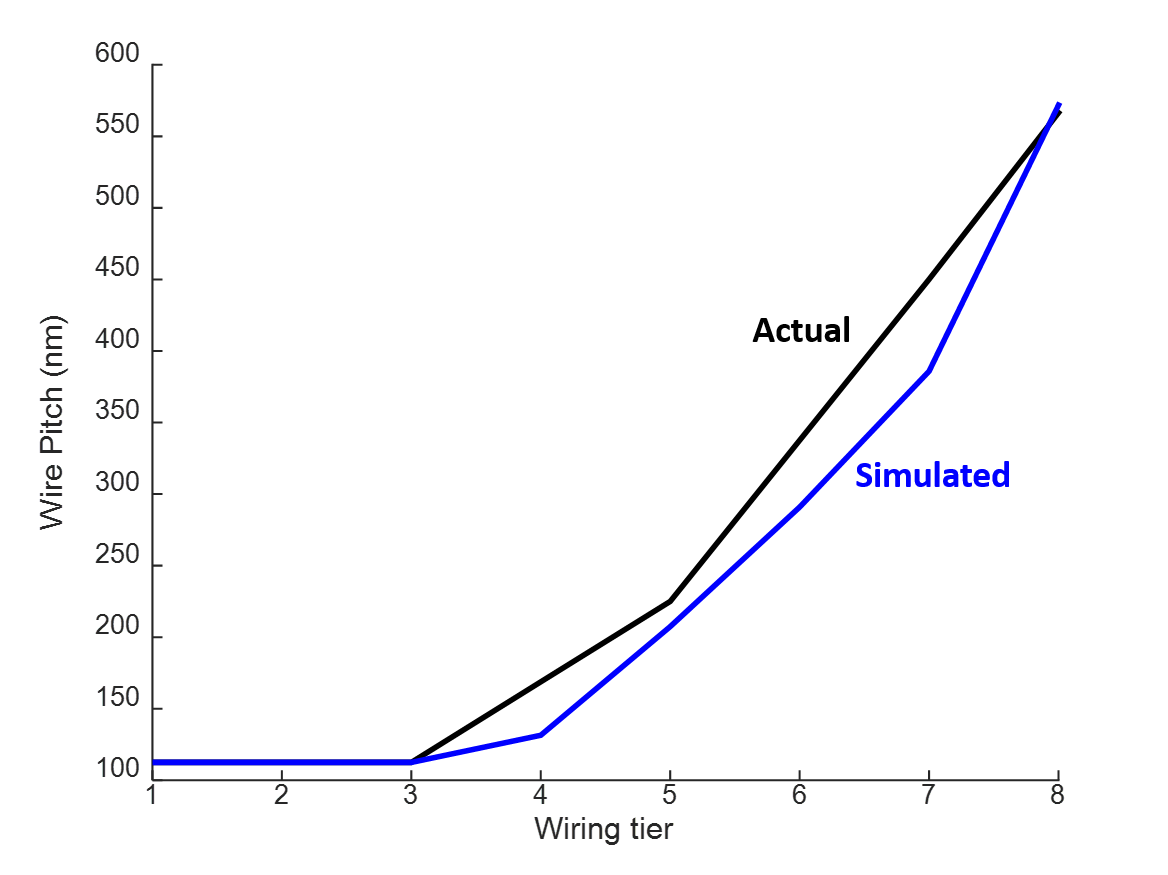
\includegraphics[width=3.5in]{Figures/sb_wire_pitch_2.png}
	\caption{
		Actual and expected wire pitch in a Core i7 2700k processor.
	}
	\label{f-sb-wire-pitch}
\end{figure}

\changed{The 45nm and 32nm test cases all have a total of 9 metal levels. In these cases the upper wiring tier has very
large wire size and pitch, and this tier is used primarily for power and clock distribution. Since the interconnect estimation
module is to estimate the size and pitch of signal wires only, the top metal layer in these designs is not counted
for the purpose of signal wire pitch validation. Rather, the pitch and size of the wires on the topmost tier is used in the.
The upper wire tier is modeled in the power delivery simulation module of the virtual platform, but without data on the
power noise margin and the number of power and ground pads used in these designs, detailed validation of the power
delivery module is not possible for these test cases.}

\begin{table}
	\centering
	%\begin{tabular}{|c|c|c|c|c|c|}
	\caption{Comparison to actual data }
	\begin{threeparttable}
	\begin{tabular}{cccccl}
		\hline
						&			&	\multicolumn{2}{c}{Signal Wire Tiers}								&	TDP		&	\multicolumn{1}{c}{Predicted} \\
		Processor		&	Node	&	Actual											&	Predicted		&	(W)		&	\multicolumn{1}{c}{Power (W)} \\
		\hline \hline
		E6850			&	65nm	&	8												&	8				&	65		&	60.27 \changed{(-7.3\%)}	\\
		E8600			&	45nm	&	\changed{8}\tnote{2}							&	8				&	65		&	63.62 \changed{(-2.1\%)}	\\
		i7 880			&	45nm	&	\changed{8}\tnote{2}							&	7				&	95		&	105.56 \changed{(11.1\%)}	\\
		i7 680\tnote{1}	&	32nm	&	\changed{8}\tnote{2}							&	6				&	73		&	52.74 \changed{(-27.8\%)}	\\
		i7 2700k		&	32nm	&	\changed{8}\tnote{2}							&	8				&	95		&	91.80 \changed{(-3.3\%)}	\\
		\hline
	\end{tabular}
	\begin{tablenotes}
		\item[1] Multi-chip package with 32nm CPU die and 45nm gpu/support die.
		\item[2] Design has one additional global metal layer for power distribution.
	\end{tablenotes}
	\end{threeparttable}
	\label{t-validation}	
\end{table}

The expected wire pitch, number of metal layers, power consumption, and
maximum junction temperature generated by the virtual platform have been compared in \cref{t-validation}. 
\changed{With the exception of the Core i7 680 test case, the virtual platform shows good agreement with the
published data for these processors. The 45nm and 32nm test cases all have a total of 9 metal layers, but in all cases
the wires on the top layer are sized very large and used for power and clock delivery, rather than signal routing.
The simulator is significantly underestimating both the number of wiring tiers
and the overall power consumption for the Core i7 680 test case; this error could be due to the fact that the
Core i7 680 is the only design under consideration which was implemented as a multi-chip module (MCM), with a CPU die (fabricated
on a 32nm process) integrated with a GPU die (fabricated on a 45nm process) in the same package.}

\changed{When simulating heterogeneous
systems, the virtual platform currently lacks the ability to estimate the power required for inter-block communication. While this
lack will affect the power estimates for all test cases, it is likely that the power required for communication between the two
separate dice in the Core i7 680 package is much larger than the power requirements for communication between GPU and logic cores
integrated on the same die (e.g. in the Sandy Bridge Core i7 2700k).}

\changed{While the worst-case error in these benchmarks is relatively high ($27.8\%$), the value of this simulation framework lies
in its ability to consider many different effects very rapidly ( a single design scenario can be evaluated in 1-5
seconds on a consumer-grade desktop or laptop computer), enabling detailed investigation of the relative performance
of different technologies on a particular design. In the subsequent sections the virtual platform is used in this manner
to investigate the impacts of material, technology, and packaging innovations on overall design quality.}

\section{2D: Seeking improvements via materials innovation} \label{s-2d-investigations}
One path towards increasing system performance is to achieve improvements in the wiring materials.
The permittivity of the interlayer dielectric (ILD) material has a strong effect on the parasitic
capacitance of the on-chip wires,
which in turn determines the RC delay and power consumption of the wiring network. In addition to
directly reducing the power required to send signals along the on-chip wires, decreasing the RC delay
also reduces the need for power-hungry repeaters.

In order to quantify this effect and to determine the potential of ultra low-k ILD materials, 
a 32nm Sandy Bridge Core i7 was simulated with a range of different
ILD permittivities, ranging from 3.9 (Silicon Dioxide), all the way down to 1 (vacuum).
Figure \ref{f-2d-materials-num-levels-ild} shows that the number of metal layers required to fully route
the Sandy Bridge processing core can be reduced from 8 to 6 if the relative dielectric constant
of the ILD material can be brought below 1.3.
The CPU power consumption scales roughly linearly with
ILD permittivity, as shown in \cref{f-2d-materials-power-consumption}, and significant power reductions
are possible with ultra low-k (ULK) materials. The power reduction comes from both a reduction in wire power,
as well as a reduction in the number and size of the repeaters needed to meet timing constraints.
While ULK dielectrics may provide one avenue towards reduced power consumption, their manufacture and integration into
the wiring stack is challenging, and poses significant reliability concerns. Alternate approaches to
reducing wire power consumption will be examined in \cref{s-3d-investigations}.

\begin{figure}[!htbp]
	\centering
	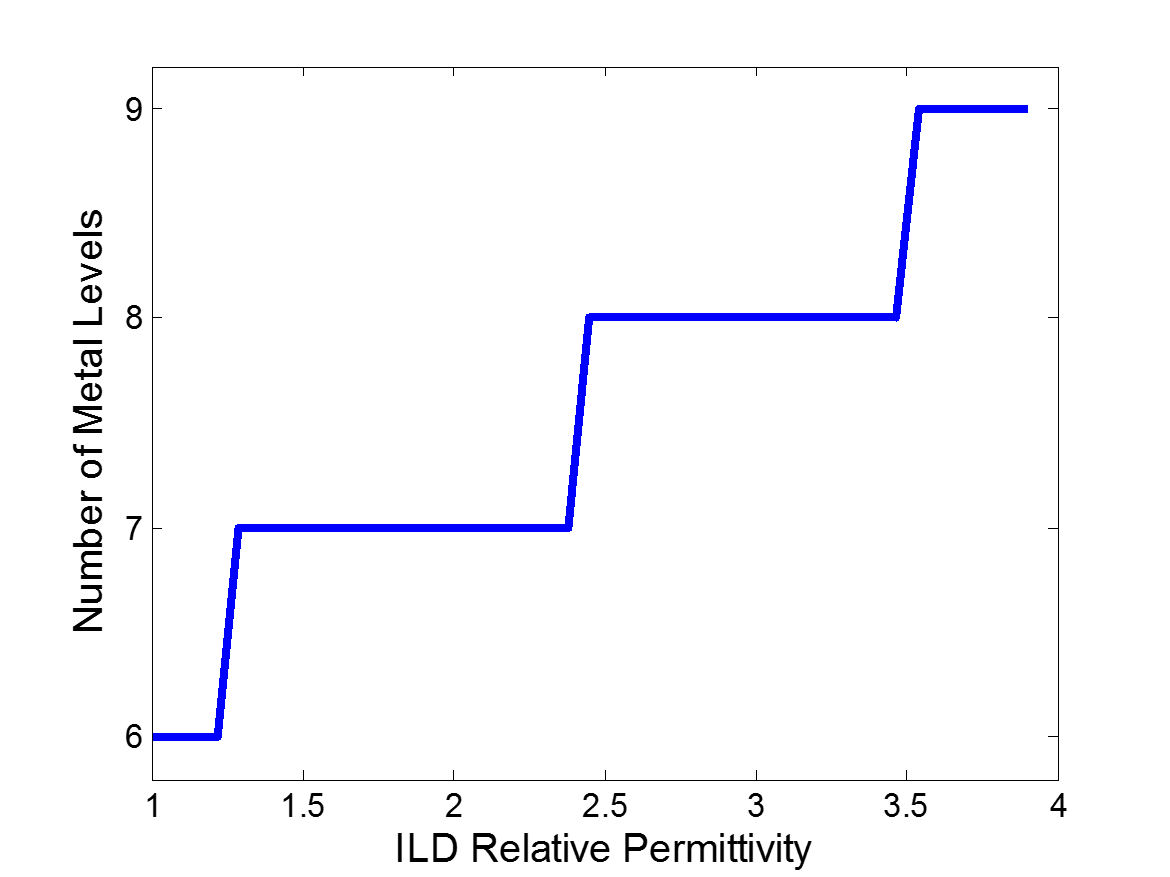
\includegraphics[width=3.5in]{Figures/sb_metal_layers_ild_eps_sweep_2.png}
	\caption{
		Impact of interlayer dielectric (ILD) permittivity on the number of metal layers required to route the wires in a Sandy Bridge Core i7 2700k.
	}
	\label{f-2d-materials-num-levels-ild}
\end{figure}

\begin{figure}[!htbp]
	\centering
	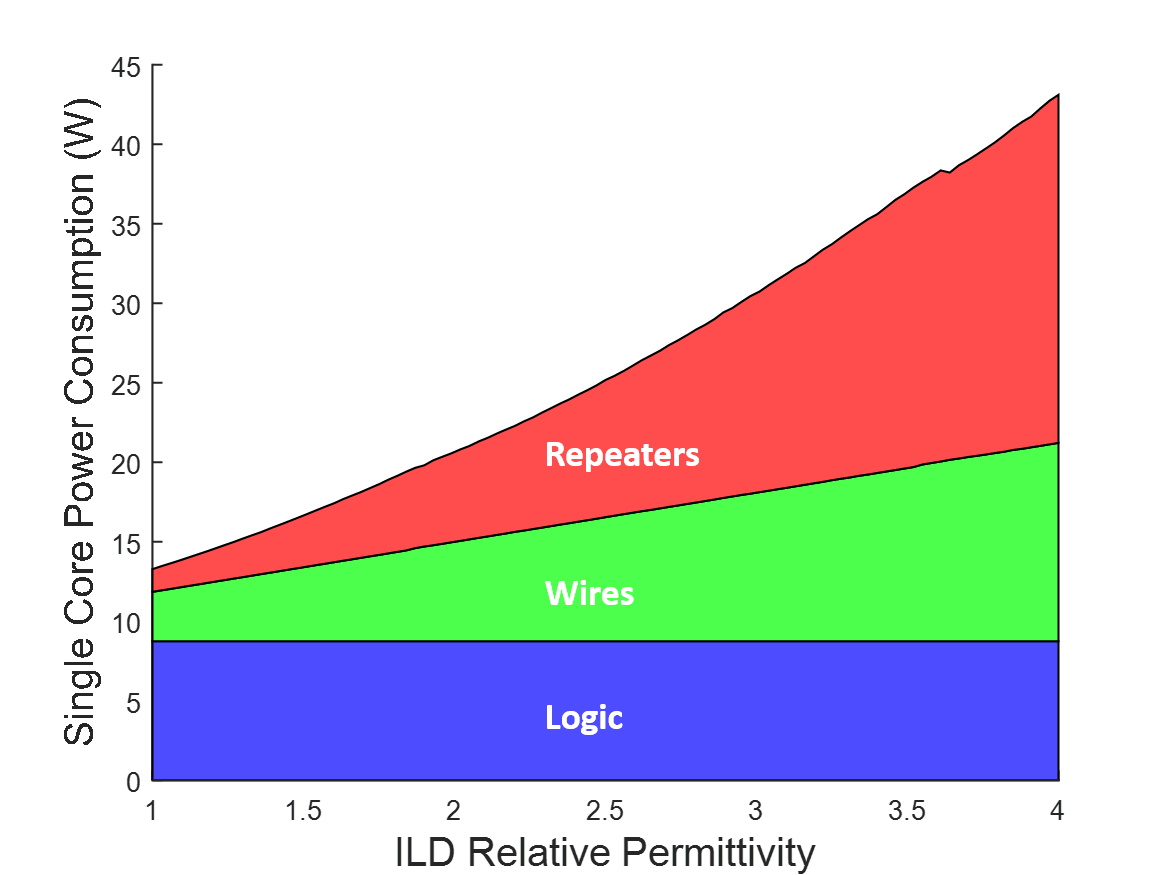
\includegraphics[width=3.5in]{Figures/total_power_sb2d_ild_permittivity_sweep_3.png}
	\caption{
		Impact of interlayer dielectric (ILD) permittivity on the power consumed by wires and repeaters in a Sandy Bridge Core i7 2700k processor core.
	}
	\label{f-2d-materials-power-consumption}
\end{figure}


The materials used for the wires must be
resistant to electromigration. As the critical dimensions of the smallest on-chip wires have decreased,
electromigration has become significant concern for system reliability at advanced process nodes 
\cite{michael_electromigration_2003,srivastava_interconnect_2004,tokei_reliability_2010}.
In order to alleviate electromigration concerns at advanced process nodes, alternate materials may be required,
which may have higher resistivities than pure copper, potentially impacting signal performance, power consumption,
and the number of metal layers required to fully route a design \cite{adelmann_alternative_2014,sankaran_exploring_2015}. % Removed sankaran_exploring_2014
It is likely that only the lowest metal levels would utilize alternate wiring materials \cite{oates-electromigration-2015,li-electromigration-2014}. 


To investigate the potential impact of electromigration-resistant metals on wire routing,
a hypothetical 7nm Sandy Bridge CPU test case was constructed by scaling the gate pitch, 
minimum wire pitch, transistor size, and all other lengths in the 32nm Sandy Bridge
by a factor of 4.57X (32/7). Two 7nm test cases were considered: \textit{7nm A}, in which all wires are composed of an
alternate material, and \textit{7nm B}, in which only wires thinner than 25nm are replaced by the alternate material.
The bulk resistivity of the alternate wiring material 
in both the 32nm and 7nm test cases was swept from 10 $\Omega$nm (slightly lower than bulk Ag), to 60 $\Omega$nm 
(slightly higher than bulk W). For simplicity, the specularity and reflection
parameters of the alternate wiring material are not modified. The results are shown in \cref{f-2d-materials-num-levels-rho-7nm}.
Since the lowest metal layers are the most critical for wire routing, small changes at these dimensions can have
a large impact on the overall wiring stack.
As can be seen in \cref{f-2d-materials-num-levels-rho-7nm}, the use of higher resistivity metals can significantly
increase the number of metal levels required for interconnect routing, but this effect can
be mitigated by restricting the use of alternate metals to the lowest wiring tiers.


\section{3D: Power reduction without exotic materials} \label{s-3d-investigations}

\subsection{Reducing power consumption}
Implementing a design in 3D can greatly reduce the average length of the on-chip interconnects,
leading to reductions in the average delay and power consumption of the signaling network \cite{joyner_impact_2001}.
In order to examine the impact of 3D integration on power consumption,
a single 18.5mm$^2$ Sandy Bridge processing core was simulated in different 3D configurations.
Unless otherwise noted, we assume a TSV aspect ratio of 20:1, and require that the TSVs use
less than 10\% of the total die area. Typically, 3DIC designs limit the TSV area to 1\% or less
to minimize the cannibalization of active area, but we have relaxed that limit here for illustrative purposes.
In order to examine the impacts of 3D integration, a single CPU core from a 32nm Sandy Bridge Core i7 2700k
is used as a test case throughout this section.

\begin{figure}[!t]
	\centering
	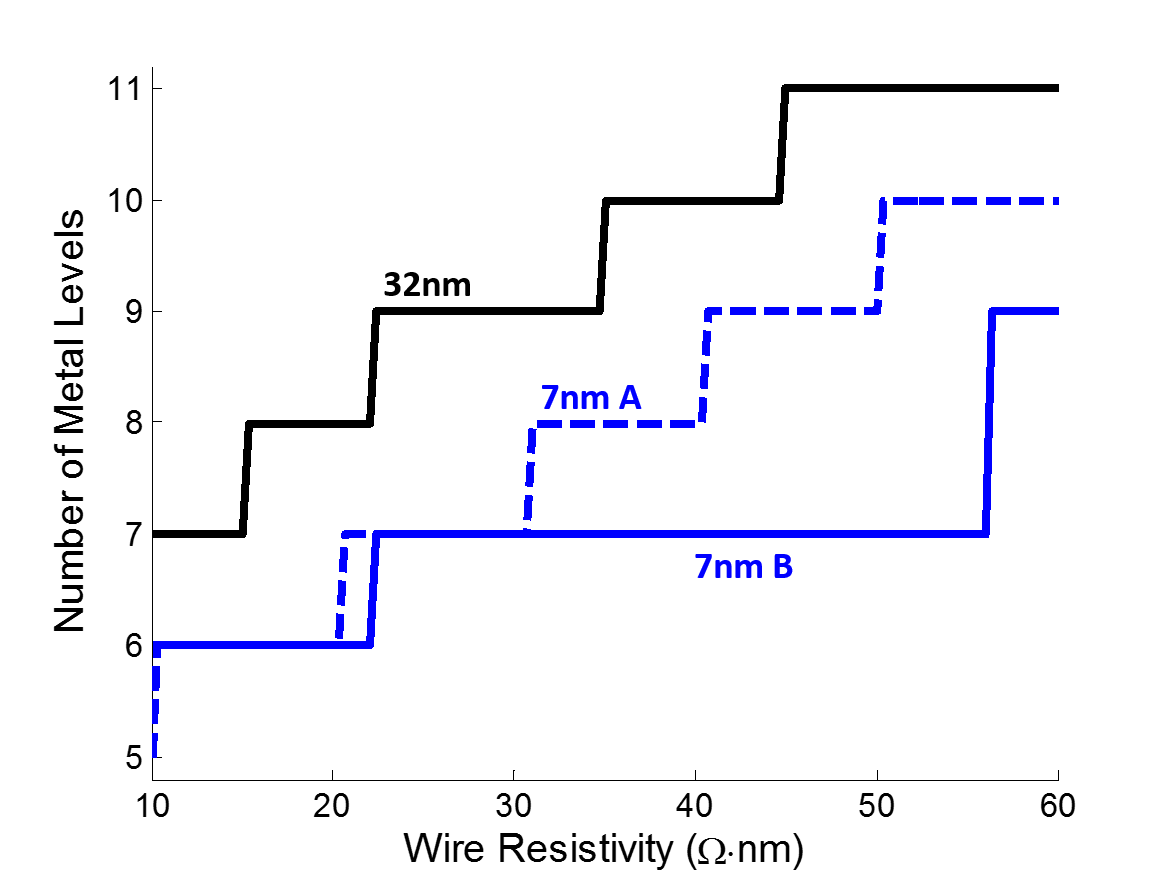
\includegraphics[width=3.5in]{Figures/sb2d_32nm_vs_7nm_alt_metal_comparison.png}
	\caption{
		Impact of wire resistivity on the number of metal layers required to route the wires in a Sandy Bridge CPU. Three cases are
		considered: a) a 32nm Sandy Bridge core; b) 7nm A, a hypothetical
		7nm Sandy Bridge core; and c) 7nm B, in which only wires with width below 25nm are modified.
	}
	\label{f-2d-materials-num-levels-rho-7nm}
\end{figure}

We consider a 3D integration scenario in which logic gates and blocks can be placed on
any tier, and in which TSVs are used as point to point interconnects.
The core is assumed to be partitioned into $N$ equal pieces, which are then stacked vertically.
This configuration is considered in order to illustrate the ultimate limits of 3D integration.

Significant power savings can be obtained by moving to a 3D design, as shown in \cref{f-sb-power-vs-tiers-ild},
though the power reduction comes at the cost of increased areal power density, ultimately placing more
stress on the cooling solution. The design implications of the increased power density of 3DICs will be discussed further
in \cref{s-3D-thermal}. It is important to note that 3DICs reduce the power required by on-chip communication, fundamentally 
improving the overall
energy efficiency of the system, as can be seen in \cref{f-sb-comm-power-fraction}.

\begin{figure}[!htbp]
	\centering
	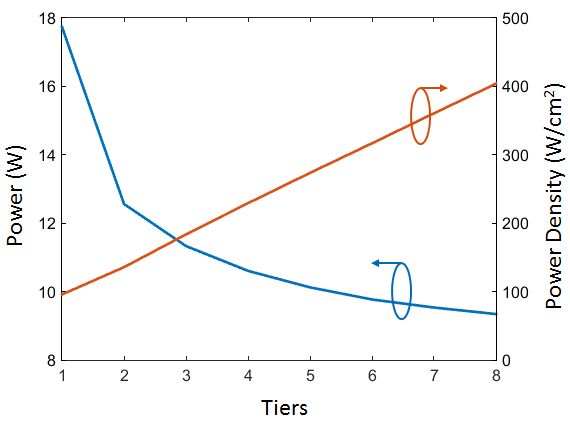
\includegraphics[width=3.5in]{Figures/sb3d_power_and_pdens2.png}
	\caption{Impact of block folding on power consumption and power density of a single 32nm Sandy Bridge core.}
	\label{f-sb-power-vs-tiers-ild}
\end{figure}

In order to fully route a 3DIC, space must be allocated on each tier for TSVs. Since TSVs consume space
that could otherwise be used for logic, it is desirable to minimize the fraction of chip area 
consumed by TSVs, to avoid unnecessarily increasing the size of each die. In order to minimize the space
occupied by TSVs, the TSV aspect ratio can either be increased, directly enabling the use of thinner TSVs,
or the die itself can be thinned, to enable the use of low aspect ratio TSVs.
Thicker logic tiers are attractive due to their higher mechanical stability, simplifying
handling and assembly, but they limit the improvement in average wire length achieved by
moving to 3D, since the distance between tiers is greater. 
TSVs are typically limited to diameters of 5-10${\mu}m$ and aspect ratios between 5-15:1 
\cite{ko_wafer-level_2012,lau_evolution_2011,dukovic_through-silicon-via_2010}, with some demonstrations of 20:1 or higher 
\cite{dembla_high_2012,fischer_very_2012,zhang_within-tier_2013}.

The impact of die thickness on 3DIC power consumption is examined in \cref{f-sb-wire-power-thickness}.
In order to realize the greatest possible power reduction from 3D integration, the active layers should be
as thin as possible, to minimize the distance that signals must travel when they are routed between tiers.

\begin{figure}[!htbp]
	\centering
	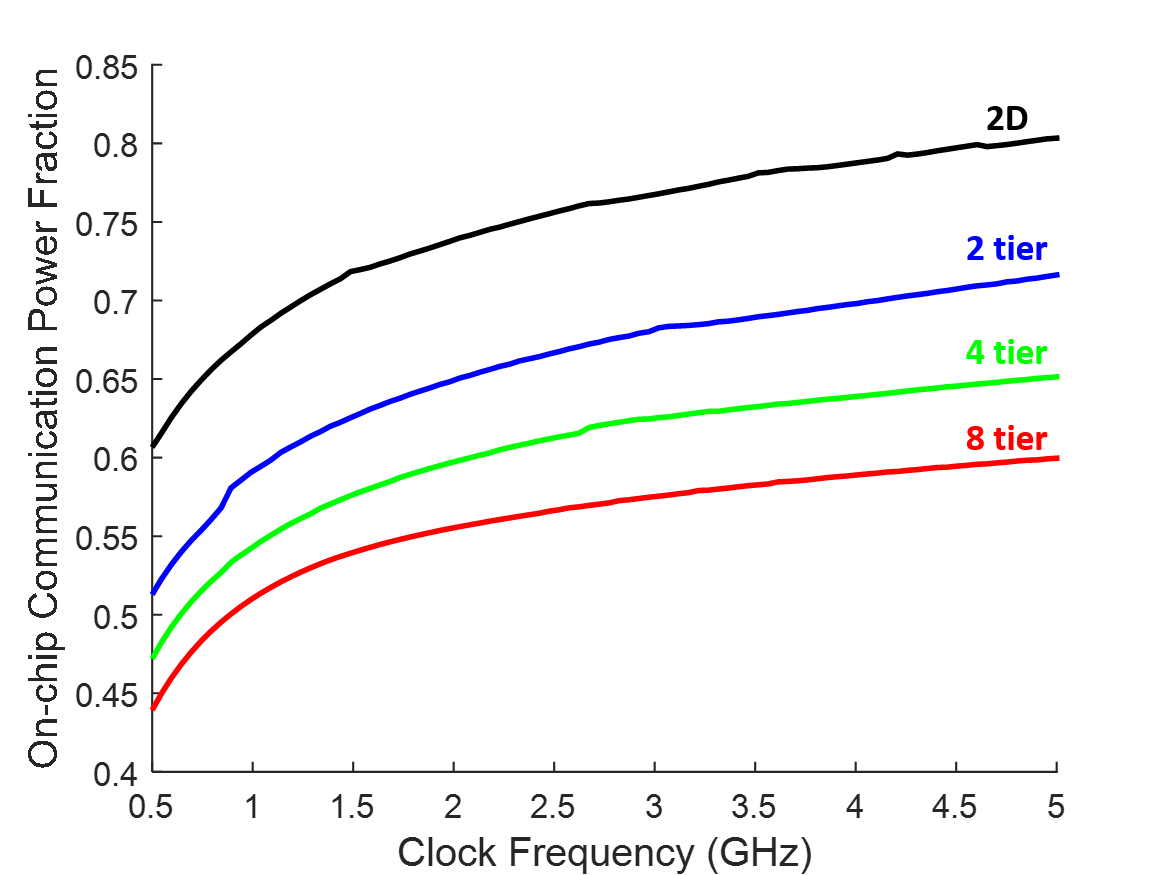
\includegraphics[width=3.5in]{Figures/sb3d_comm_power_fraction_4.png}
	\caption{Fraction of power consumed for on-chip communication as a function of 3D configuration and operating frequency.}
	\label{f-sb-comm-power-fraction}
\end{figure}

\begin{figure}[!htbp]
	\centering
	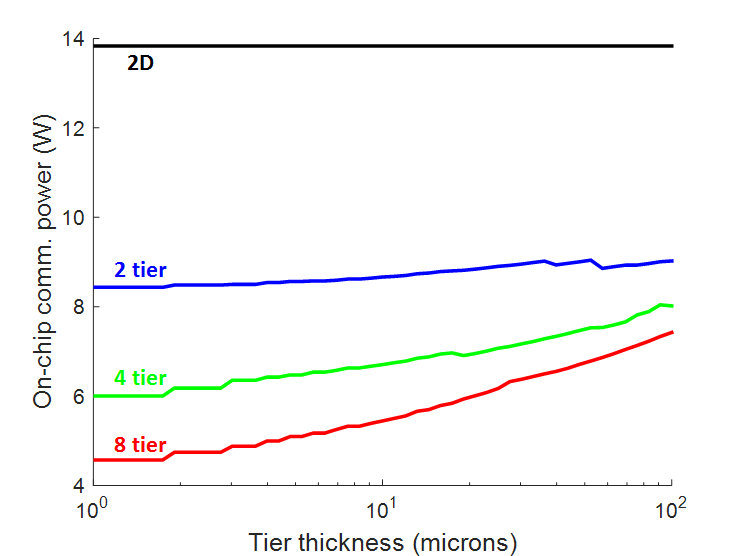
\includegraphics[width=3.5in]{Figures/sb3d-comm-power-vs-thickness_3.png}
	\caption{Impact of die thickness on power consumed by wires and repeaters in a single 32nm Sandy Bridge core implemented in 3D.}
	\label{f-sb-wire-power-thickness}
\end{figure}

\subsection{Power Delivery}
In order for an IC to function reliably,
the power delivery network must be robust enough to prevent undue fluctuation of the supply voltage \cite{huang_power_2012}.
Power delivery becomes more challenging as the power density that must be delivered increases.
Power delivery in 3DICs becomes especially challenging, as a high performance 3DIC may have a significantly
higher areal power density than an equivalent 2D chip, while simultaneously having less space available for
routing power delivery resources. Additionally, in 3DICs power must be delivered to each tier in the stack
through TSVs, introducing additional parasitic resistance and inductance into the wiring network.

The most straightforward way to ease the burden on the power network is to reduce the total power consumption of the system.
The total power consumption of an IC can be reduced by moving to a 3D configuration, though the 
areal power density increases as more tiers are stacked atop one another.
As the power density increases, delivering power to all of the tiers of the 3D stack
becomes more challenging, and many TSVs may be required to minimize droop in the
supply voltage of advanced 3DICs.
Silicon area is already a limited resource, and the tradeoff between allocating TSVs for signaling
or power delivery must be managed carefully.

The number of power connections to each tier required for stable operation is primarily determined by the maximum power draw of the system,
which in turn is strongly dependent upon the interlayer dielectric and the substrate thickness (in 3D configurations).
Both 2D and 3D systems benefit from the development of ultralow-k interlayer dielectric materials, and 
the use of thin substrates in 3D configurations can further reduce the demands on the power supply network.

In order to
explore these effects, the Sandy Bridge test case was simulated with several substrate thicknesses and interlayer
dielectric permittivities, in order to determine the number of power delivery pads or TSVs needed to reduce
the simultaneous switching noise to below 15\% of the nominal supply voltage. The results are presented in \cref{f-3d-psn-ild-tiers}.
For two-tier stacks only a slight increase in power TSVs is observed over the 2D case, but
the eight-tier implementation requires roughly an order of magnitude
more power connections than the 2D design. The dielectric constant of the ILD material has a strong impact on the power delivery requirements,
as it has an outsized impact on the power consumption of the on-chip communication network. The thickness 
of the 3DIC logic tiers is not a limiting factor for 2-tier designs, but 4- and 8-tier designs can realize nearly as much benefit
from extreme die thinning as from the use of ultralow-k dielectrics.

Another method to reduce the power supply noise is to integrate decoupling capacitors onto the die, interposer, or package
in order to compensate for the inductance of the power delivery network. While this practice can improve
power quality, it also sets up a tradeoff between utilizing die area for logic, decoupling capacitors, and power delivery.

In order to explore this tradeoff, the 32nm Sandy Bridge test case was simulated in several 2D and 3D configurations with
varying amounts of silicon area allocated for chip- or interposer-level 
decoupling capacitors. The power TSV diameter is assumed to be 10 ${\mu}m$ and the thickness of each die in the 3D stack is assumed to be
10 ${\mu}m$ \changed{to investigate the potential of extreme die thinning. While processing and assembling thinned wafers can be challenging,
alternate integration schemes in which wafers are bonded and subsequently thinned could enable the stacking of such thin layers
without the need for modified wafer handling processes \cite{patti-three-dimensional-2006}}.
As can be seen in \cref{f-sb-psn-decap-10um}, increasing the decoupling
capacitance can significantly reduce the number of pads or TSVs required for power delivery.
Small area allocations can likely be achieved
with on-chip decoupling capacitors, but integrating more than several square millimeters of decoupling capacitors
into a 2D or 3D system will likely require the use of either a dedicated capacitor tier, or interposer-based
decoupling capacitors. Even with the use of decoupling capacitors, a lower bound on power TSV number is set by
the need to keep the current density carried by each TSV low enough to avoid electromigration effects.

\begin{figure}[!htbp]
	\centering
	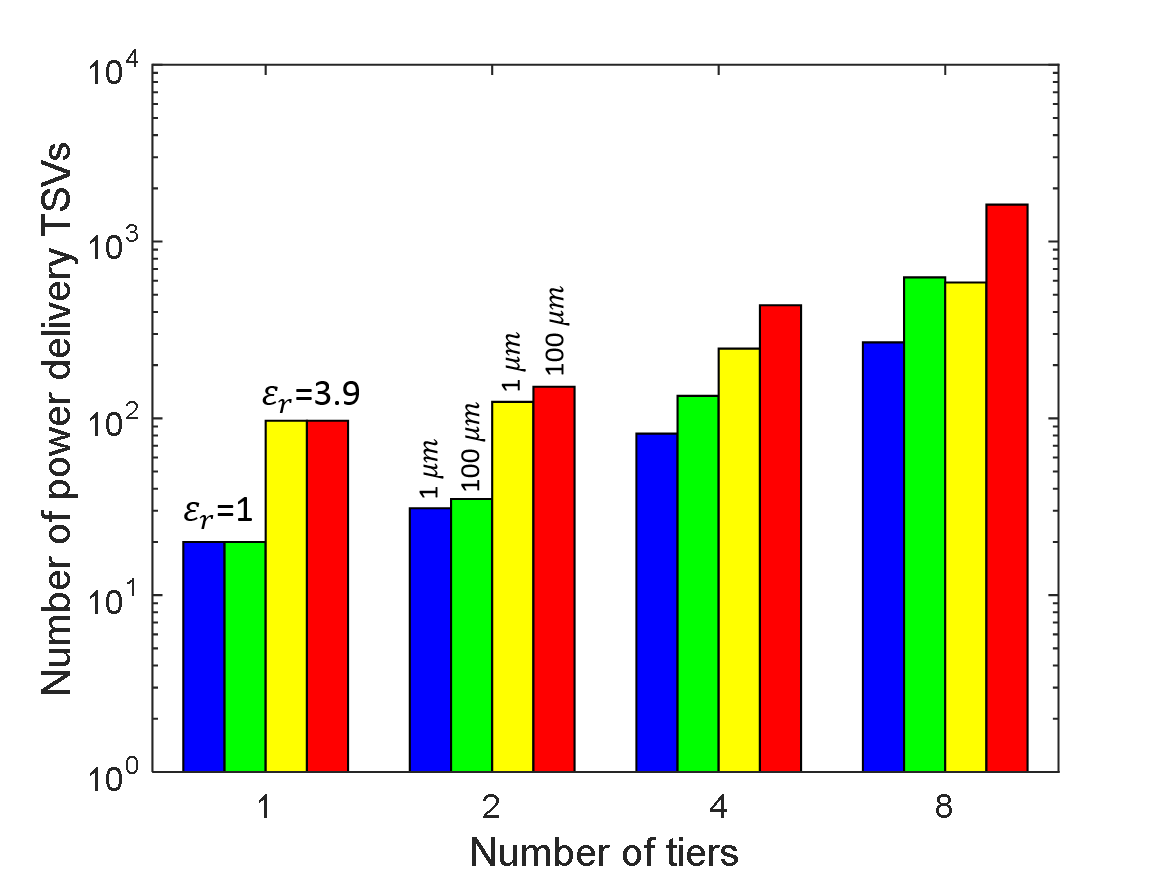
\includegraphics[width=3.5in]{Figures/sb3d_psn_vs_ild_and_tiers_vacuum_vs_sio2_3.png}
	\caption{
		Impact of interlayer dielectric material, substrate thickness, and degree of 3D 
		integration on power delivery TSV requirements in a hypothetical 3D Sandy Bridge CPU core.
		In the single-tier (2D) case the required number of power pads is displayed.
	}
	\label{f-3d-psn-ild-tiers}
\end{figure}

\begin{figure}[!htbp]
	\centering
	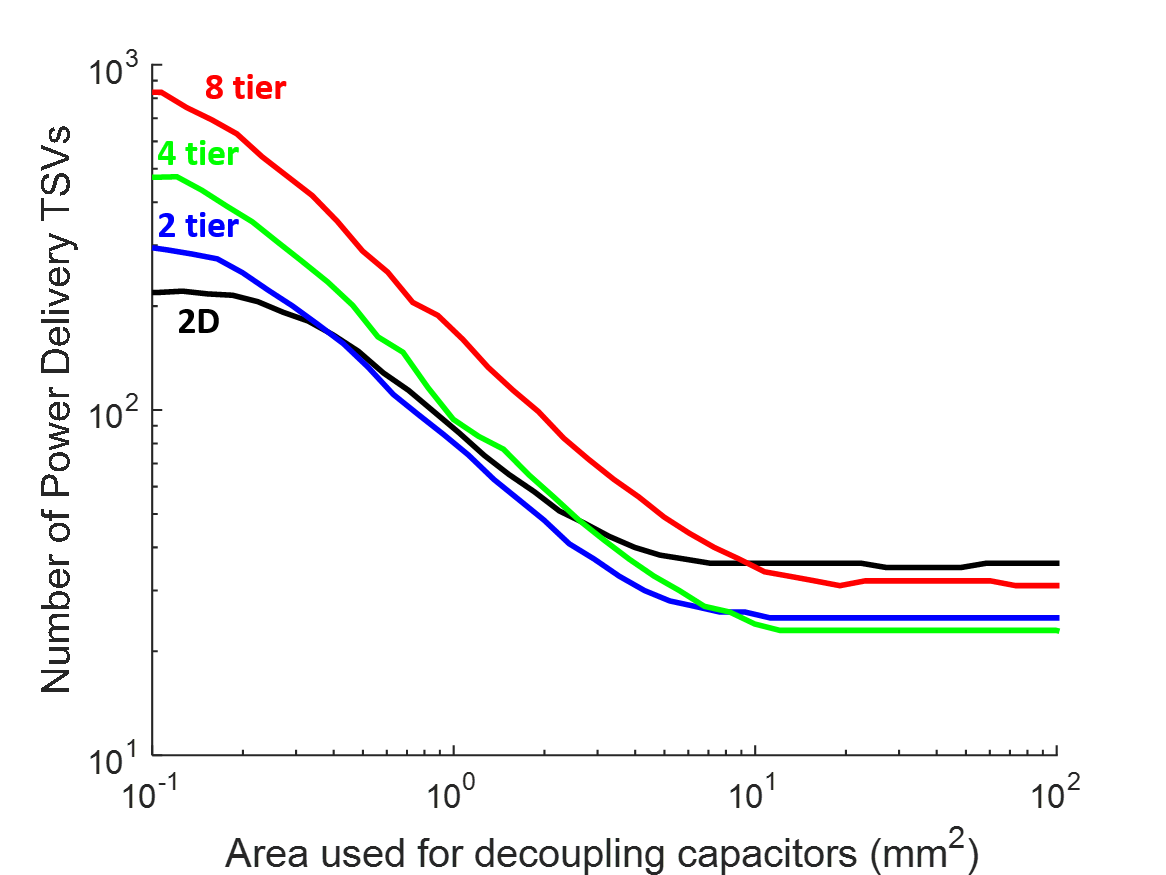
\includegraphics[width=3.5in]{Figures/sb3d_psn_tiers_and_decap__substrate_10um__tsvs_10um_3.png}
	\caption{
		Power TSV requirements for a single Sandy Bridge core as a function of 3D configuration and
		area allocated for decoupling capacitors.
		}
	\label{f-sb-psn-decap-10um}
\end{figure}

\subsection{Thermal management} \label{s-3D-thermal}
Thermal management is a key challenge for 3DICs. In the previous sections it has been shown that transforming a
2D design into a 3DIC can yield significant reductions in the average wire length and power consumption of the system,
and the use of ultrathin active layers has been shown to further reduce the power consumption of 3DICs.
Additionally, low-k dielectrics can be used to decrease the power consumption of the on-chip communication network in
both 2D and 3D systems.

While the total power dissipation of an IC is expected to decrease as the device is partitioned into increasing numbers of layers 
(as shown in \cref{f-sb-power-vs-tiers-ild}),
that power reduction is not sufficient to keep the areal power density from increasing as tiers are stacked atop one another,
leading to increased stress on the cooling system, and eventually to unreasonable operating temperatures. Since most
conventional 2D ICs are already operating at their thermal limits, a system transformed from 2D to 3D must necessarily either
run at a lower operating frequency, or utilize a more aggressive cooling solution.

In order to quantify these tradeoffs, the performance of a single 32nm Sandy Bridge CPU core is examined in several configurations:
\begin{enumerate}
	\item 2D and 3D configurations are investigated to demonstrate the impact of 3D integration on system performance.
	\item The relative permittivity of the ILD material is swept from 1.0 (vacuum) to 3.9 (silicon dioxide) in order
			to illustrate the impact of ULK materials on system performance
	\item Air cooling and microfluidic water cooling are compared in order to demonstrate the benefits of aggressive heat removal techniques.
			Heat sink parameters are taken from \cite{zhang-micropinfin-heat-sink-2013}
\end{enumerate}
The CPU core was simulated in each configuration to find 
the maximum operating frequency which could be maintained while keeping the maximum temperature below 90$^\circ$C.
As can be seen in \cref{f-3d-fmax-comparison}, the maximum frequency decreases rapidly as the CPU is folded across
more and more tiers, as the increased power density of the system increases the strain on the cooling system.
The power consumption each core remains essentially constant for the entire range
of dielectric constants, as the maximum temperature in the stack is primarily a function of the areal power dissipation
of the system and the thermal parameters of the heat sink used. The thermally-limited power draw for each configuration 
is shown in \cref{f-3d-pmax-air-vs-water}.

\begin{figure}[!htbp]
	\centering
	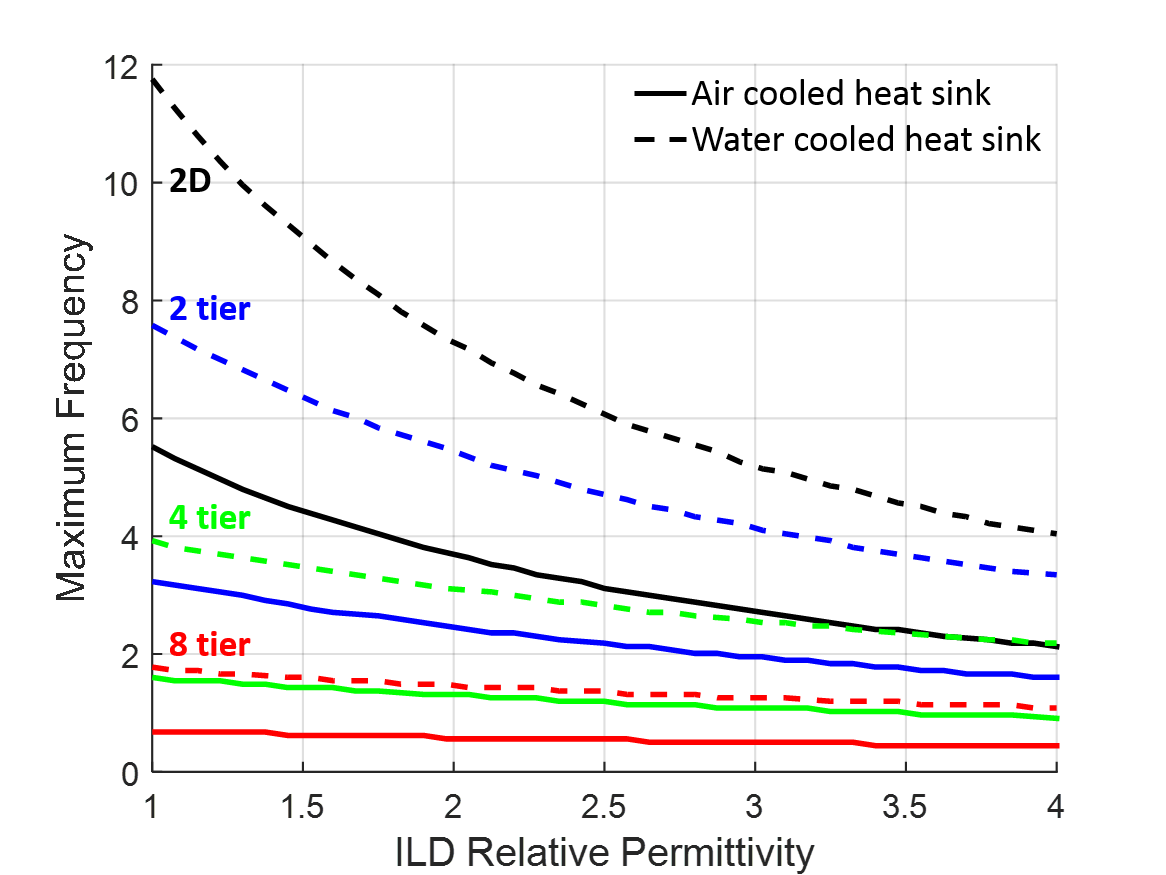
\includegraphics[width=3.5in]{Figures/SB3D_max_frequency__aircooled_watercooled__ILD_Sweep_2.png}
	\caption{
		Maximum operating frequency the Sandy Bridge processing core can achieve while keeping the maximum junction temperature below 90$^\circ$C.
		Solid lines correspond to air cooling, and dashed lines correspond to water cooling.
		}
	\label{f-3d-fmax-comparison}
\end{figure}

\begin{figure}[!htbp]
	\centering
	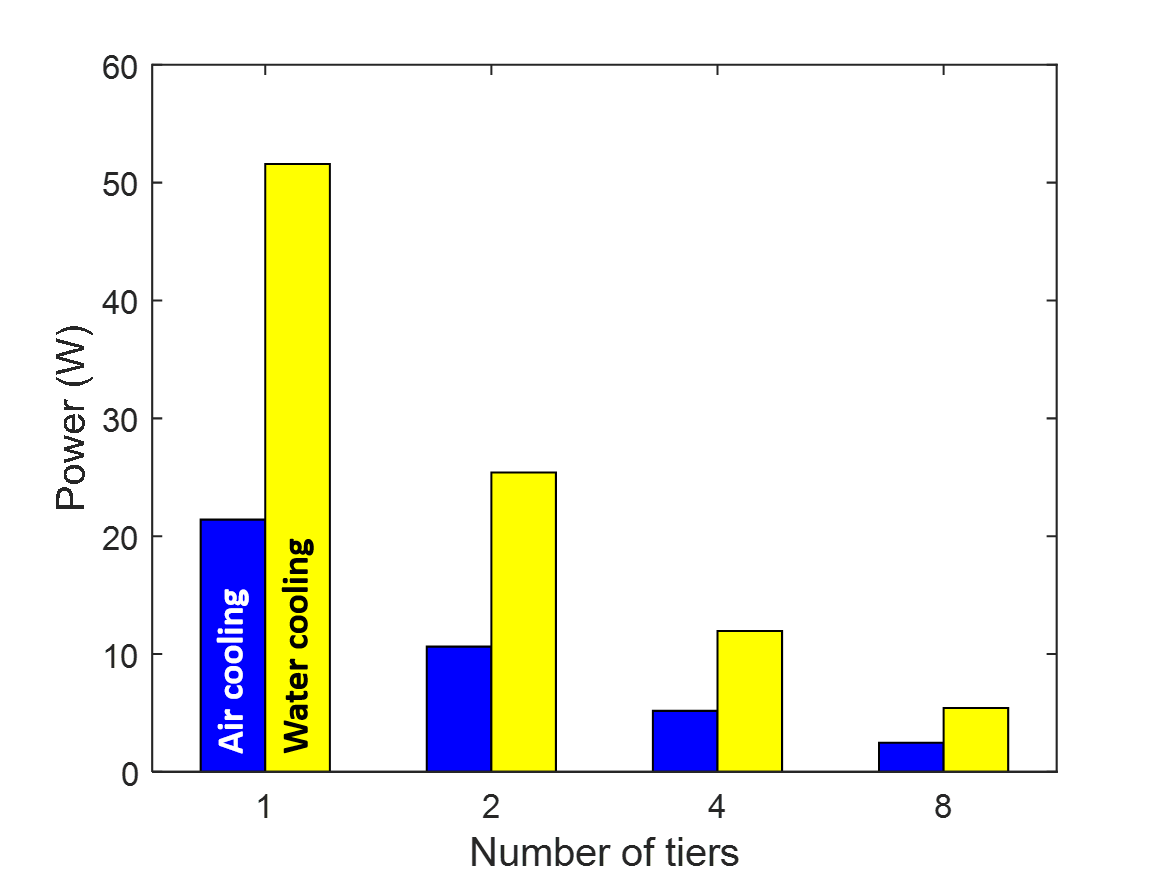
\includegraphics[width=3.5in]{Figures/sb3d_air_vs_water_power_consumption.png}
	\caption{
		Maximum power consumption of 2D and 3D Sandy Bridge CPU cores limited to 90$^\circ$C with air cooling (blue) and water cooling (yellow).
		}
	\label{f-3d-pmax-air-vs-water}
\end{figure}

While the water-cooled designs can be run faster than air-cooled designs, they typically sacrifice 
energy efficiency for performance,
as shown in \cref{f-3d-epc-air-vs-water}. Water-cooled CPU cores folded over four or more tiers, however, are projected
to exhibit equal or better EPC as their air-cooled counterparts, due to the combination of the significant communication power savings
benefit from 3D integration and the performance enhancement afforded by effective heat removal from the 3D stack. 
In all cases, reducing the dielectric constant of the ILD material can significantly decrease the power consumption of 
the CPU core, yielding a significant performance benefit for thermally-limited systems.

\begin{figure}[!htbp]
	\centering
	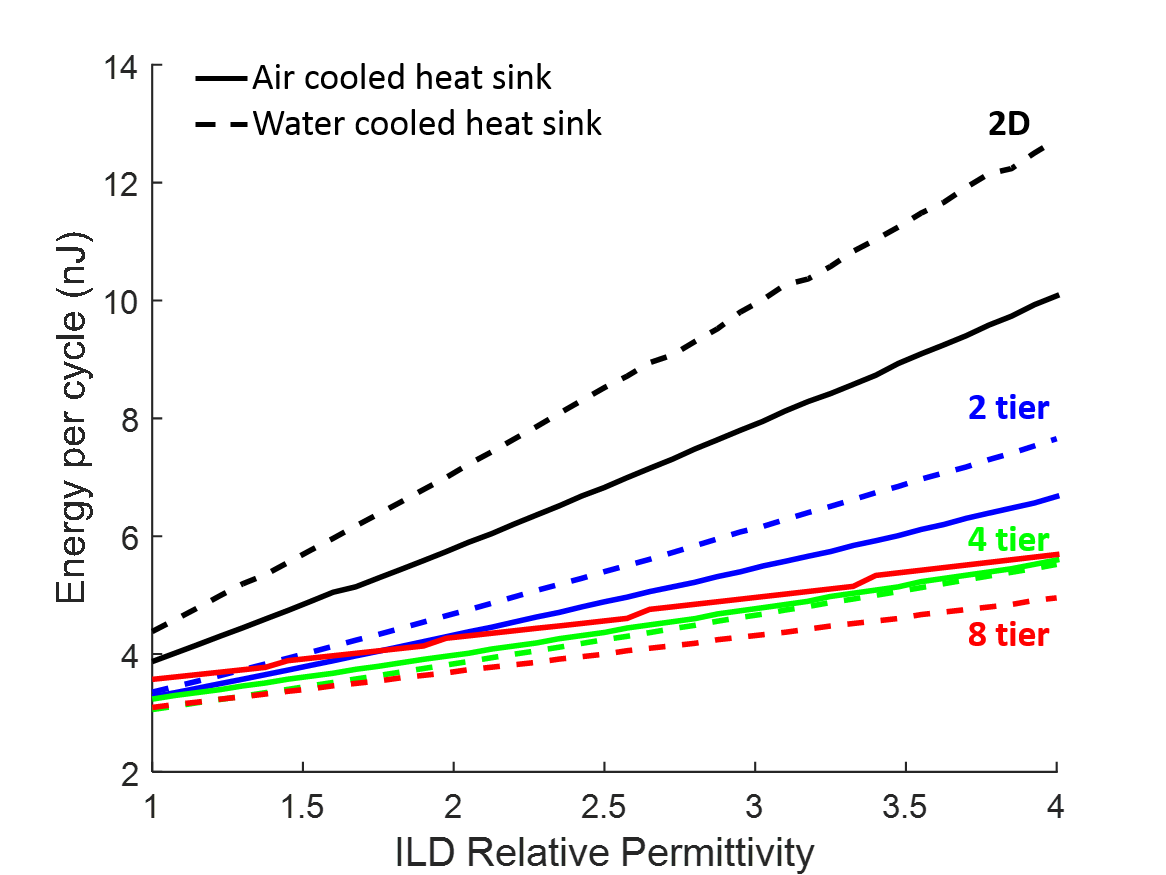
\includegraphics[width=3.5in]{Figures/sb3d_air_vs_water_energy_per_cycle.png}
	\caption{
		Energy consumption per clock cycle for 2D and 3D Sandy Bridge CPU cores limited to 90$^\circ$C with air-cooled (solid lines) and water-cooled (dashed lines) heat sinks.
		}
	\label{f-3d-epc-air-vs-water}
\end{figure}


%% =================================
%% ========= CONCLUSION ============
%% =================================

\section{Conclusion}
A virtual integration platform for 2D and 3D IC pathfinding was developed and used to examine the impacts of 
advanced technologies on system performance. The virtual platform incorporates 
models for signal delivery, power supply noise, and thermal performance in 2D and 3D ICs,
and was validated against wire pitch and power consumption data for recent commercial microprocessors.
The impacts of 
low-k dielectrics, and 3D integration on the performance, power consumption,
and power delivery requirements of a 32nm processing core were examined, and a hypothetical 7nm version of the same processor
was simulated to determine the impact of alternate wire materials on the number of metal levels required for signal routing
at advanced process nodes.





\section*{Acknowledgments}
The authors gratefully acknowledge the support of the Semiconductor
Research Corporation Global Research Collaboration (task ID 2254.001),
as well as the SRC Educational Alliance Intel Foundation Fellowship.

%% Fiddle with this to manually align columns on last page
%\enlargethispage{-1.0in}


%% Include bibliography
\bibliographystyle{IEEEtran_local}

% Use this to manually decrease the effective page size to balance the bibliography columns.
%May not work in all IEEE modes.
%\IEEEtriggercmd{\enlargethispage{-1.0in}} 

%% Use this to break the references at a particular reference number (don't use with enlargethispage)
%\IEEEtriggeratref{26}

% Start the bibliography!
\bibliography{references}

\begin{IEEEbiography}[{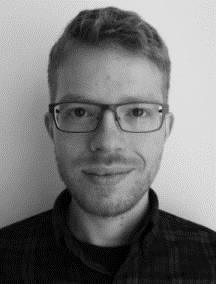
\includegraphics[width=1in,height=1.25in,clip,keepaspectratio]{Figures/bio-will.png}}]%
{William Wahby}
(S13) received the B.S. and M.S. degrees in electrical and computer engineering from the
University of Illinois at Urbana Champaign,
Urbana, IL, USA, in 2007 and 2009, respectively. He worked
as a Product Engineer at Intel until 2011, when he
joined the Ph.D. program in electrical
and computer engineering at the Georgia Institute
of Technology. In 2014 he received the SRC Education Alliance
Intel Foundation Fellowship.
His research interests include 3DIC
performance modeling, monolithic 3D integration, chip-scale optical interconnects, 
and novel memory devices.
\end{IEEEbiography}

%\vspace{-0.3in}

\begin{IEEEbiography}[{
\includegraphics[width=1in,height=1.25in,clip,keepaspectratio]{Figures/bio-li.png}}]%
{Li Zheng}
received the B.S. degree from Zhejiang
University, Hangzhou, China, in 2006, and the dual
M.S. degree in electrical and computer engineering
from Shanghai Jiao Tong University, Shanghai,
China, and the Georgia Institute of Technology,
Atlanta, GA, USA, in 2009, where he is currently
pursuing the Ph.D. degree in electrical and computer
engineering.
His current research interests include embedded
microfluidic cooling, power delivery modeling
and chip-to-chip signaling modeling for high performance
silicon interposer, and 3-D integrated systems.
\end{IEEEbiography}


%\vspace{-0.3in}


\begin{IEEEbiography}[{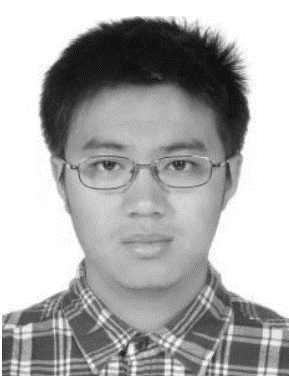
\includegraphics[width=1in,height=1.25in,clip,keepaspectratio]{Figures/bio-yang.png}}]%
{Yang Zhang}
(S�13) received the B.S. degree
in microelectronics and mathematics from Peking
University, Beijing, China, in 2012. He is currently
pursuing the Ph.D. degree in electrical engineering
with the Georgia Institute of Technology, Atlanta,
GA, USA.
\end{IEEEbiography}




%\vfill
%\newpage


\begin{IEEEbiography}[{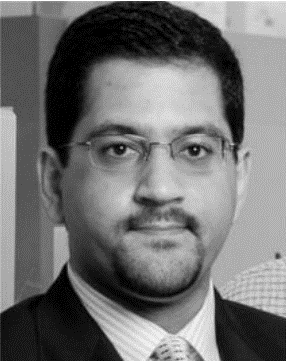
\includegraphics[width=1in,height=1.25in,clip,keepaspectratio]{Figures/bio-muhannad.png}}]%
{Muhannad S. Bakir}
(SM�12) received the B.E.E.
(summa cum laude) degree from Auburn University,
Auburn, AL, USA, in 1999, and the M.S. and Ph.D.
degrees in electrical and computer engineering from
the Georgia Institute of Technology (Georgia Tech),
Atlanta, GA, USA, in 2000 and 2003, respectively.
He is currently an Associate Professor and the
ON Semiconductor Junior Professor with the School
of Electrical and Computer Engineering at Georgia
Tech.
Dr. Bakir is an Editor of the IEEE TRANSACTIONS
ON ELECTRON DEVICES, an Associate Editor of the IEEE TRANSACTIONS
ON COMPONENTS, PACKAGING AND MANUFACTURING TECHNOLOGY, and
was a Guest Editor of the June 2011 special issue of the IEEE Journal
of Selected Topics in Quantum Electronics. He is also a member of the
International Technology Roadmap for Semiconductors� technical working
group for assembly and packaging. He was a recipient of the 2013 Intel
Early Career Faculty Honor Award, the 2012 DARPA Young Faculty Award,
the 2011 IEEE CPMT Society Outstanding Young Engineer Award, and was
an Invited Participant in the 2012 National Academy of Engineering Frontiers
of Engineering Symposium. He was also a recipient of the Semiconductor
Research Corporation�s Inventor Recognition Awards in 2002, 2005, and 2009.
He and his research group have received 12 conference and student paper
awards, including one from the IEEE Custom Integrated Circuits Conference,
five from the IEEE Electronic Components and Technology Conference, and
three from the IEEE International Interconnect Technology Conference.
\end{IEEEbiography}



%\vfill


\end{document}
